\chapter[Introduction]


%==================================================================================================
\section{Introduction}

%--------------------------------------------------------------------------------------------------
\subsection{Motivation}
I have encountered a problem that was insipration for this work during my research in field
of mobile robotics. While my initial focus was directed more towards emergent behaviour in 
robotics and a self organizing systems I have encountered a issue with localization in marine 
robotics. With high cost of internet connection for robots operating far away from land it 
is important to be able to calculate precise position without updating data from internet.
One of issuse when working with satellite navigation system is requirement for clock bias
correction, to keep error drift to minimum readouts for both local and satellite clock must
be corrected by predicted bias. In this work I focused on prediction of errors in satellite
clocks as unlike in case of local clock those can be later reused by other people.


%--------------------------------------------------------------------------------------------------
\subsection{History of robotics}

%--------------------------------------------------------------------------------------------------
\subsection{Acknoweledgements}

%==================================================================================================
\section{Robot navigation}

%--------------------------------------------------------------------------------------------------
\subsection{Basic concepts}
Unlike a robotic manipulators for which there is always a single joint fixed to a specific
location in external reference frame mobile robot must be equipped with a way to localize
themselves in environment.
\begin{figure}[hb]
	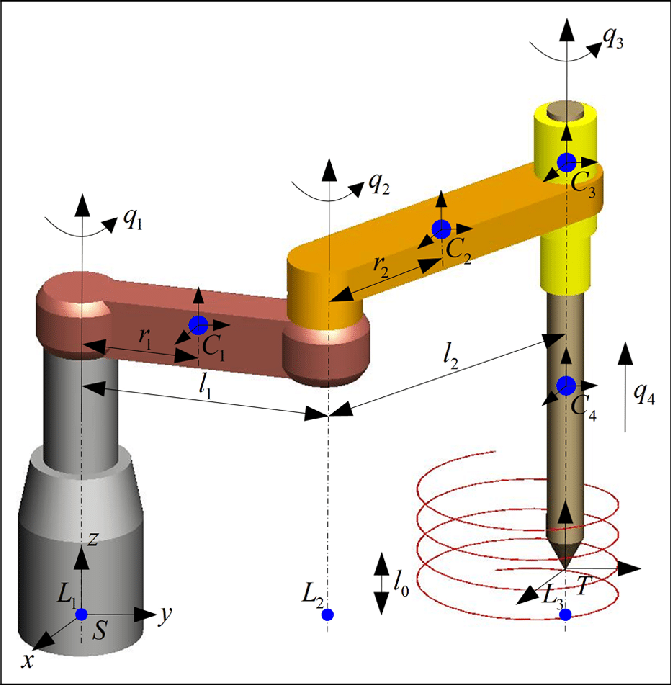
\includegraphics[width=0.5\textwidth]{robot_arm_reference}
	\caption{Kinematic chain of robotic manipulatr}
	\label{fig:robot_arm_reference}
\end{figure}


%--------------------------------------------------------------------------------------------------
\subsection{Reference versus dead reckoning}

%--------------------------------------------------------------------------------------------------
\subsection{Beacon based navigation}


%==================================================================================================
\section{Global navigation satellite systems}

%--------------------------------------------------------------------------------------------------
\subsection{GPS}

%--------------------------------------------------------------------------------------------------
\subsection{GLONASS}

%--------------------------------------------------------------------------------------------------
\subsection{Galileo}

%--------------------------------------------------------------------------------------------------
\subsection{Others}




